\begin{qu}[Two charged rods]\num
In figure A, a charged rod acts on a charged ball from a certain
distance. In B, two such rods act from twice the distance on the same ball.

\vspace{20mm}

\includegraphics{electromagnetism/figs/two-rods-double-distance}

\noindent The deflections $\theta_A$ and $\theta_B$ of the strings from the vertical are

A. equal

B. unequal, with $\theta_A < \theta_B$

C. unequal, with $\theta_A > \theta_B$

D. need more information

\end{qu}
